\chapter{Figures}

\vspace*{-3in}


\begin{figure}
\vspace{2.4in}
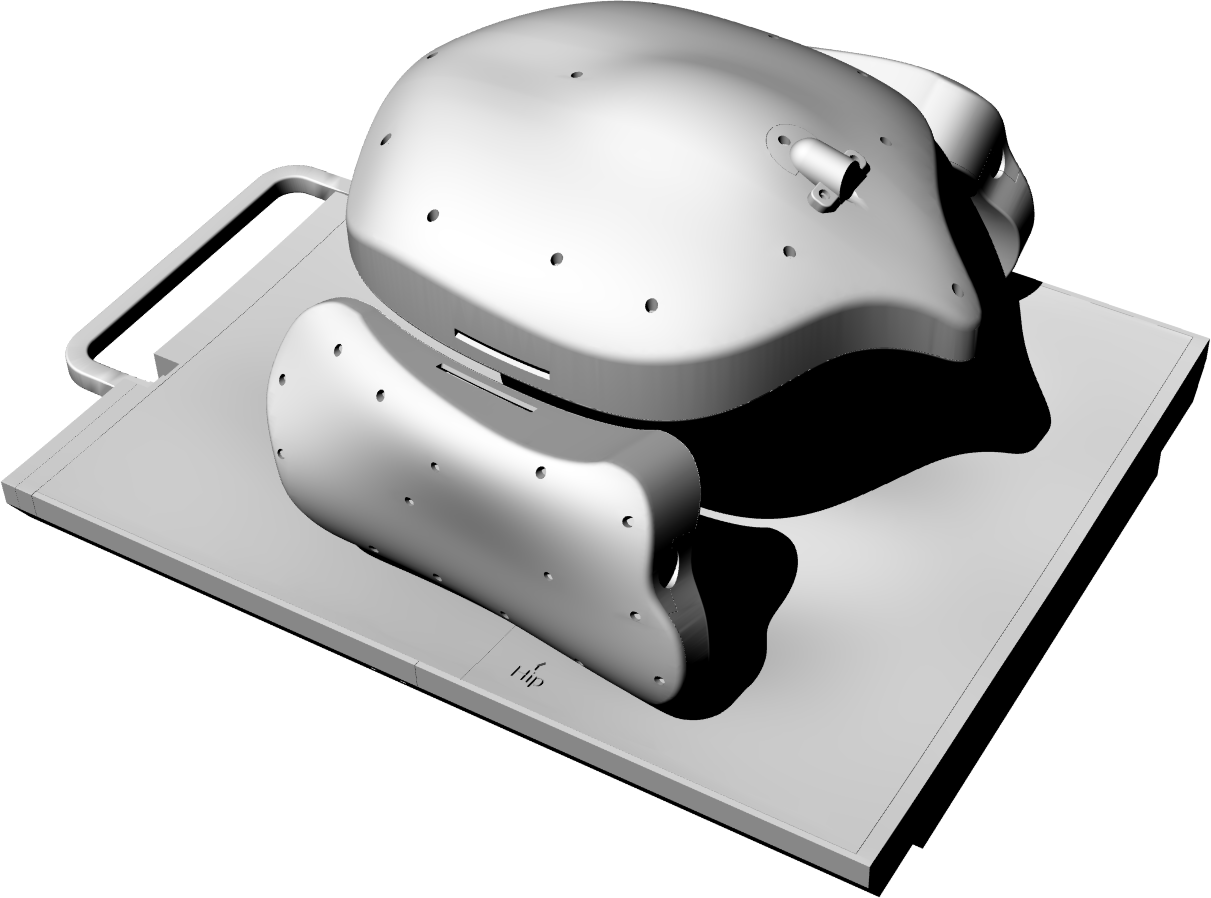
\includegraphics[width=6in]{figures/cad_rendering.png}
\caption{Computer rendering of array panels and housings}
\label{fig:cad_rendering}
\end{figure}
\clearpage
\newpage

\begin{figure}
\vspace{2.4in}
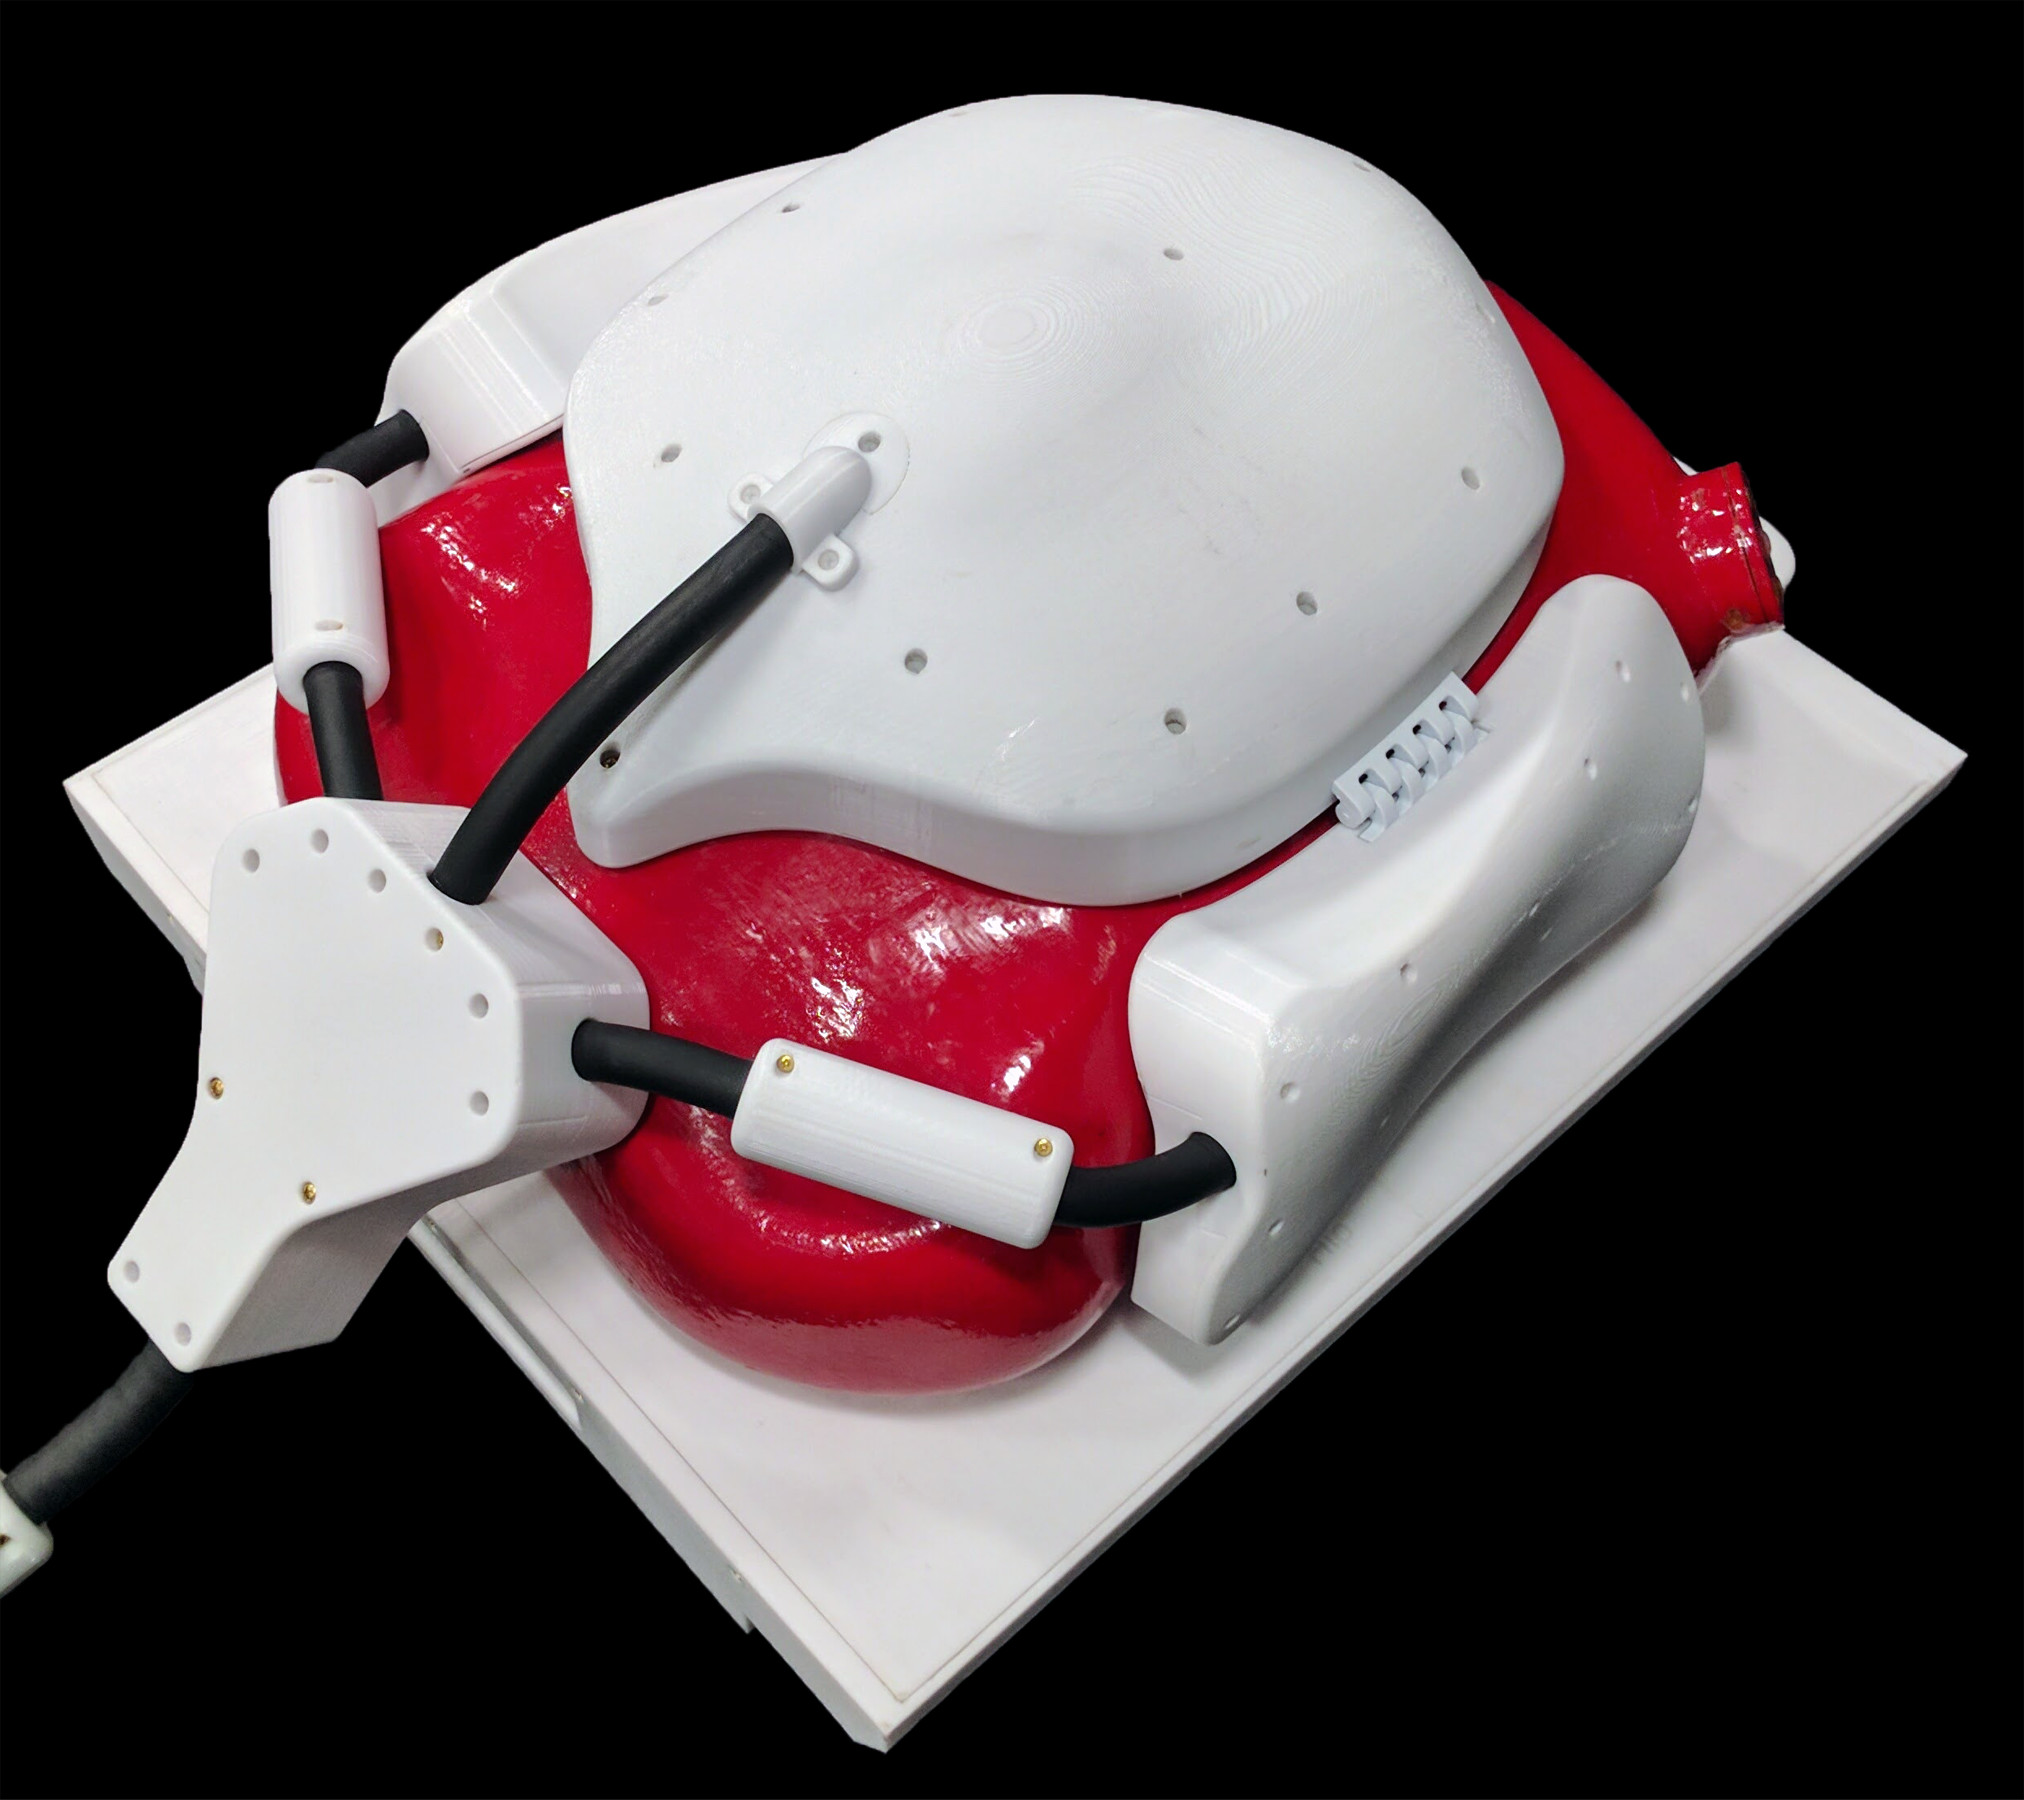
\includegraphics[width=6in]{figures/assembled_view.jpg}
\caption{Finished coil, posed on 22 week pregnant abdomen phantom}
\label{fig:assembled_view}
\end{figure}
\clearpage
\newpage

\begin{figure}
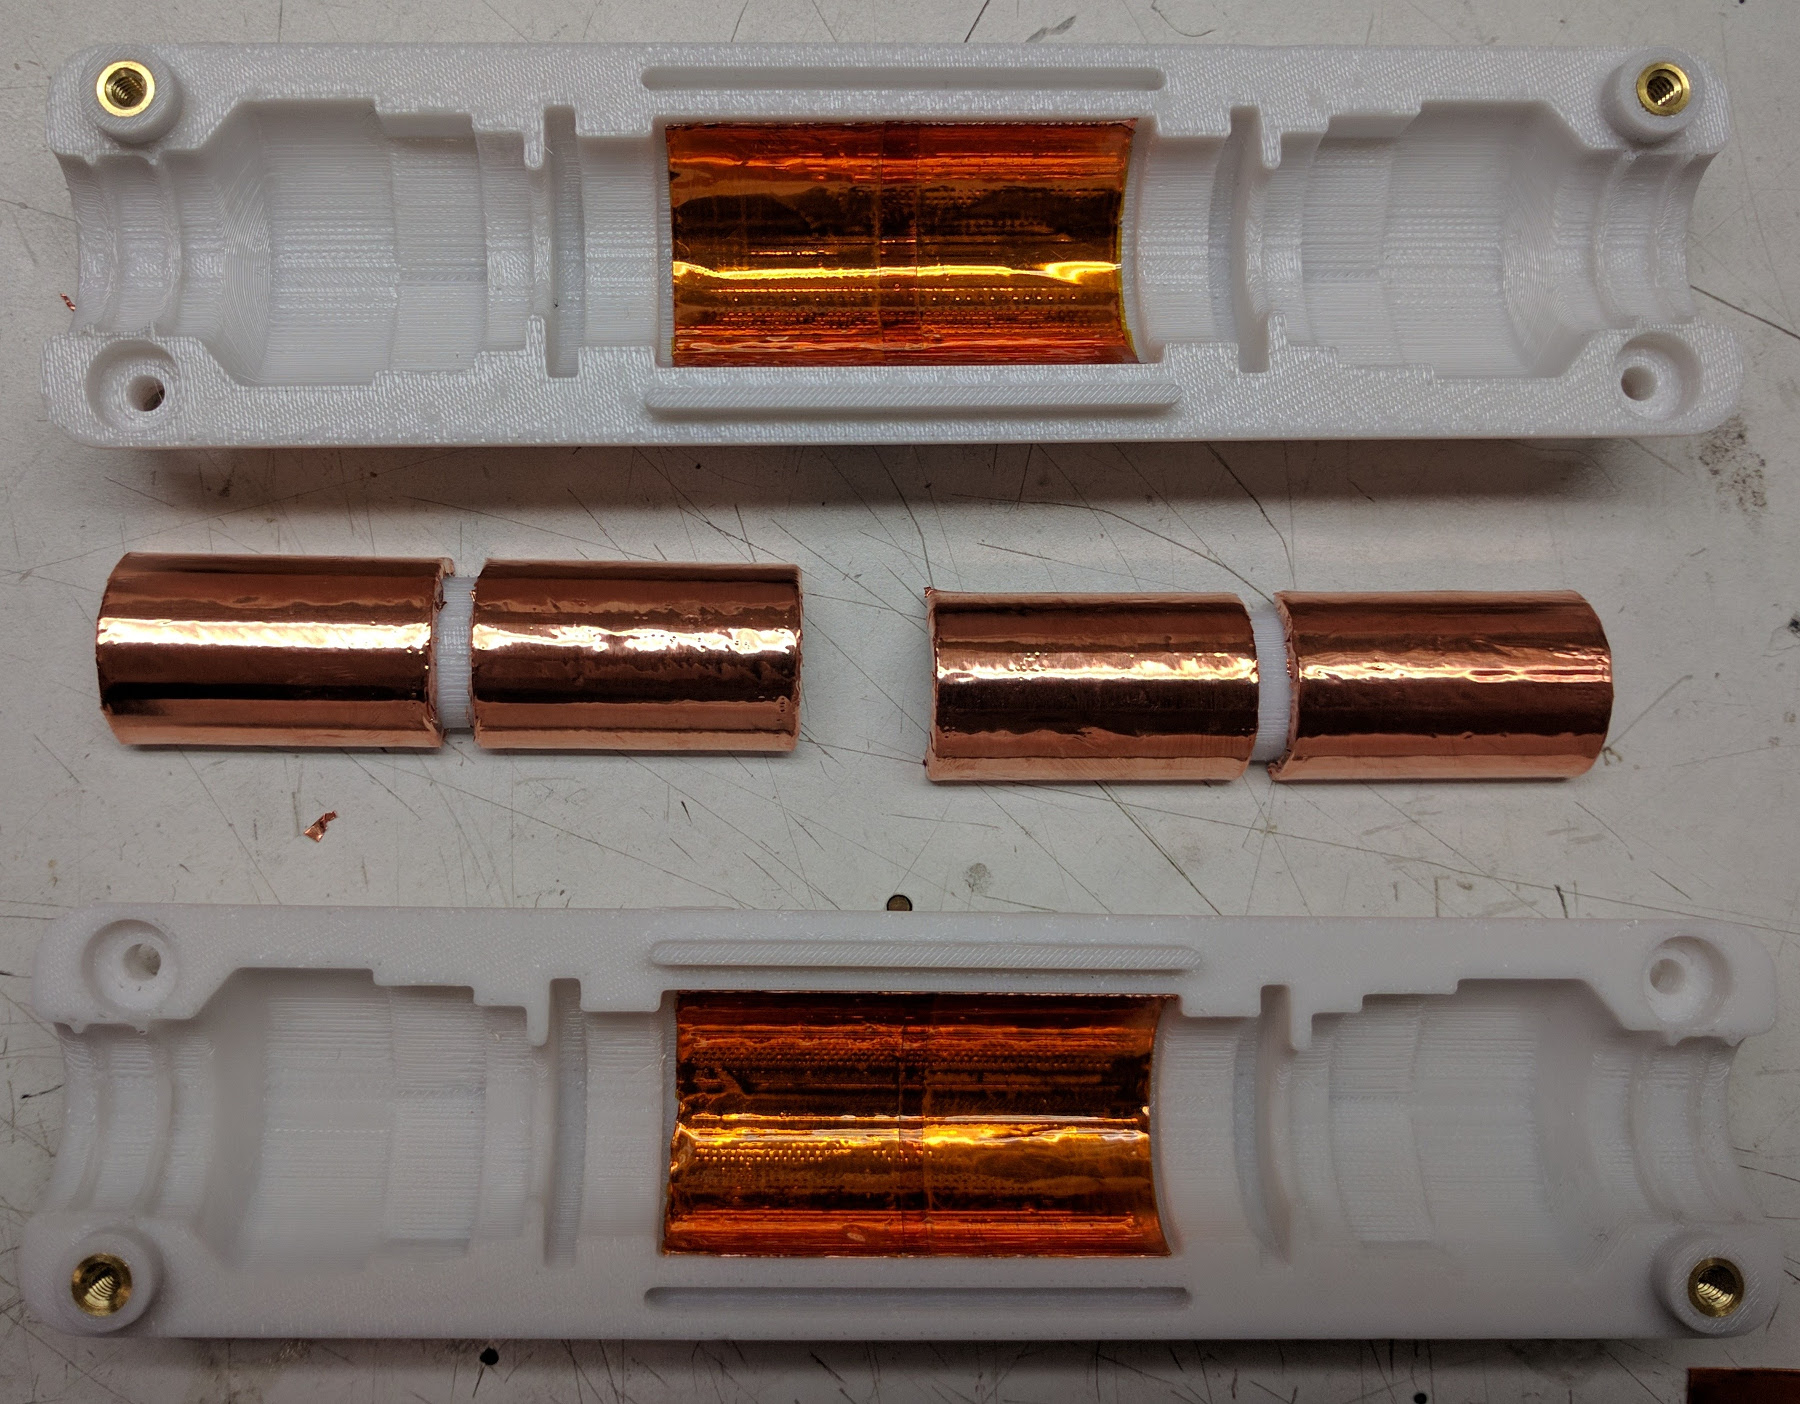
\includegraphics[width=6in]{figures/bazooka_parts.jpg}
\caption{Bazooka Balun before assembly}
\label{fig:bazooka_parts}
\end{figure}

\begin{figure}
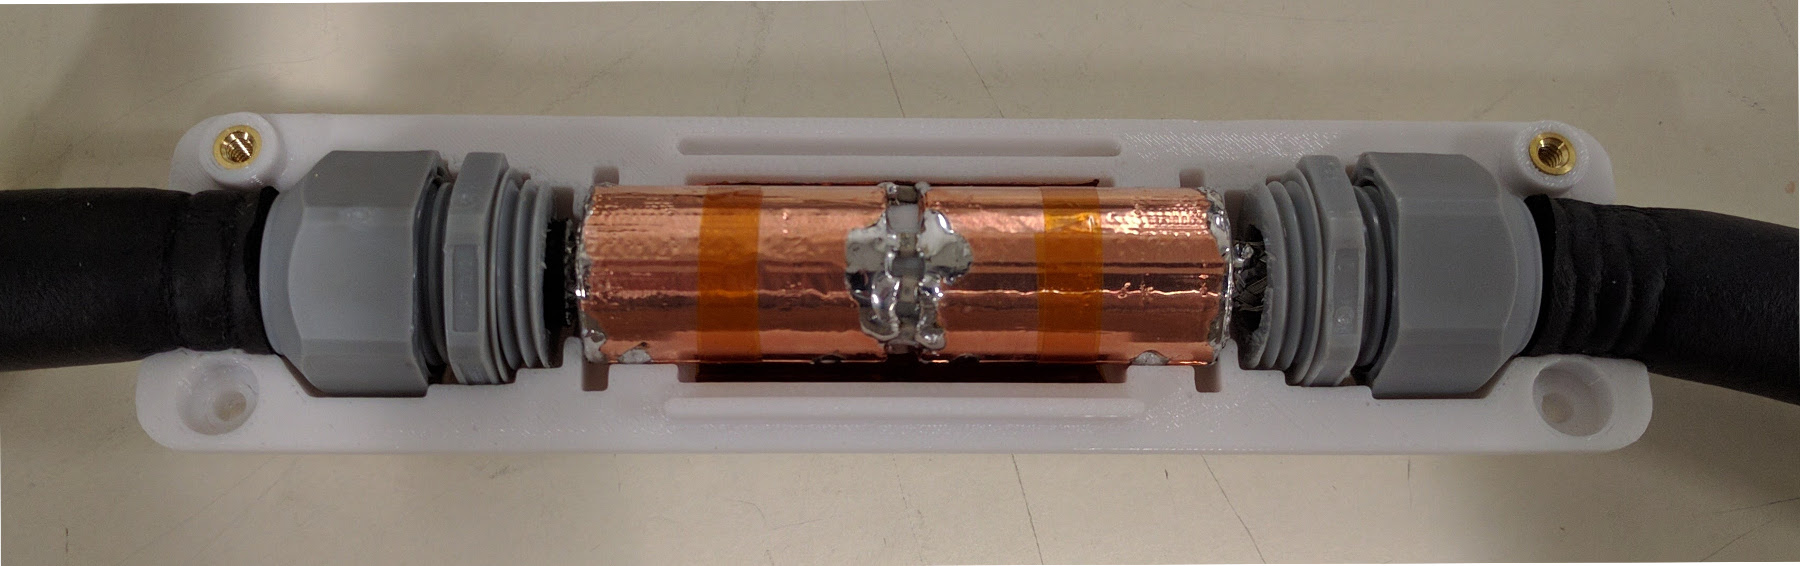
\includegraphics[width=6in]{figures/bazooka_assembled.jpg}
\caption{Completed bazooka balun with open enclosure}
\label{fig:bazooka_assembled}
\end{figure}
\clearpage
\newpage

\begin{figure}
\vspace{2.4in}
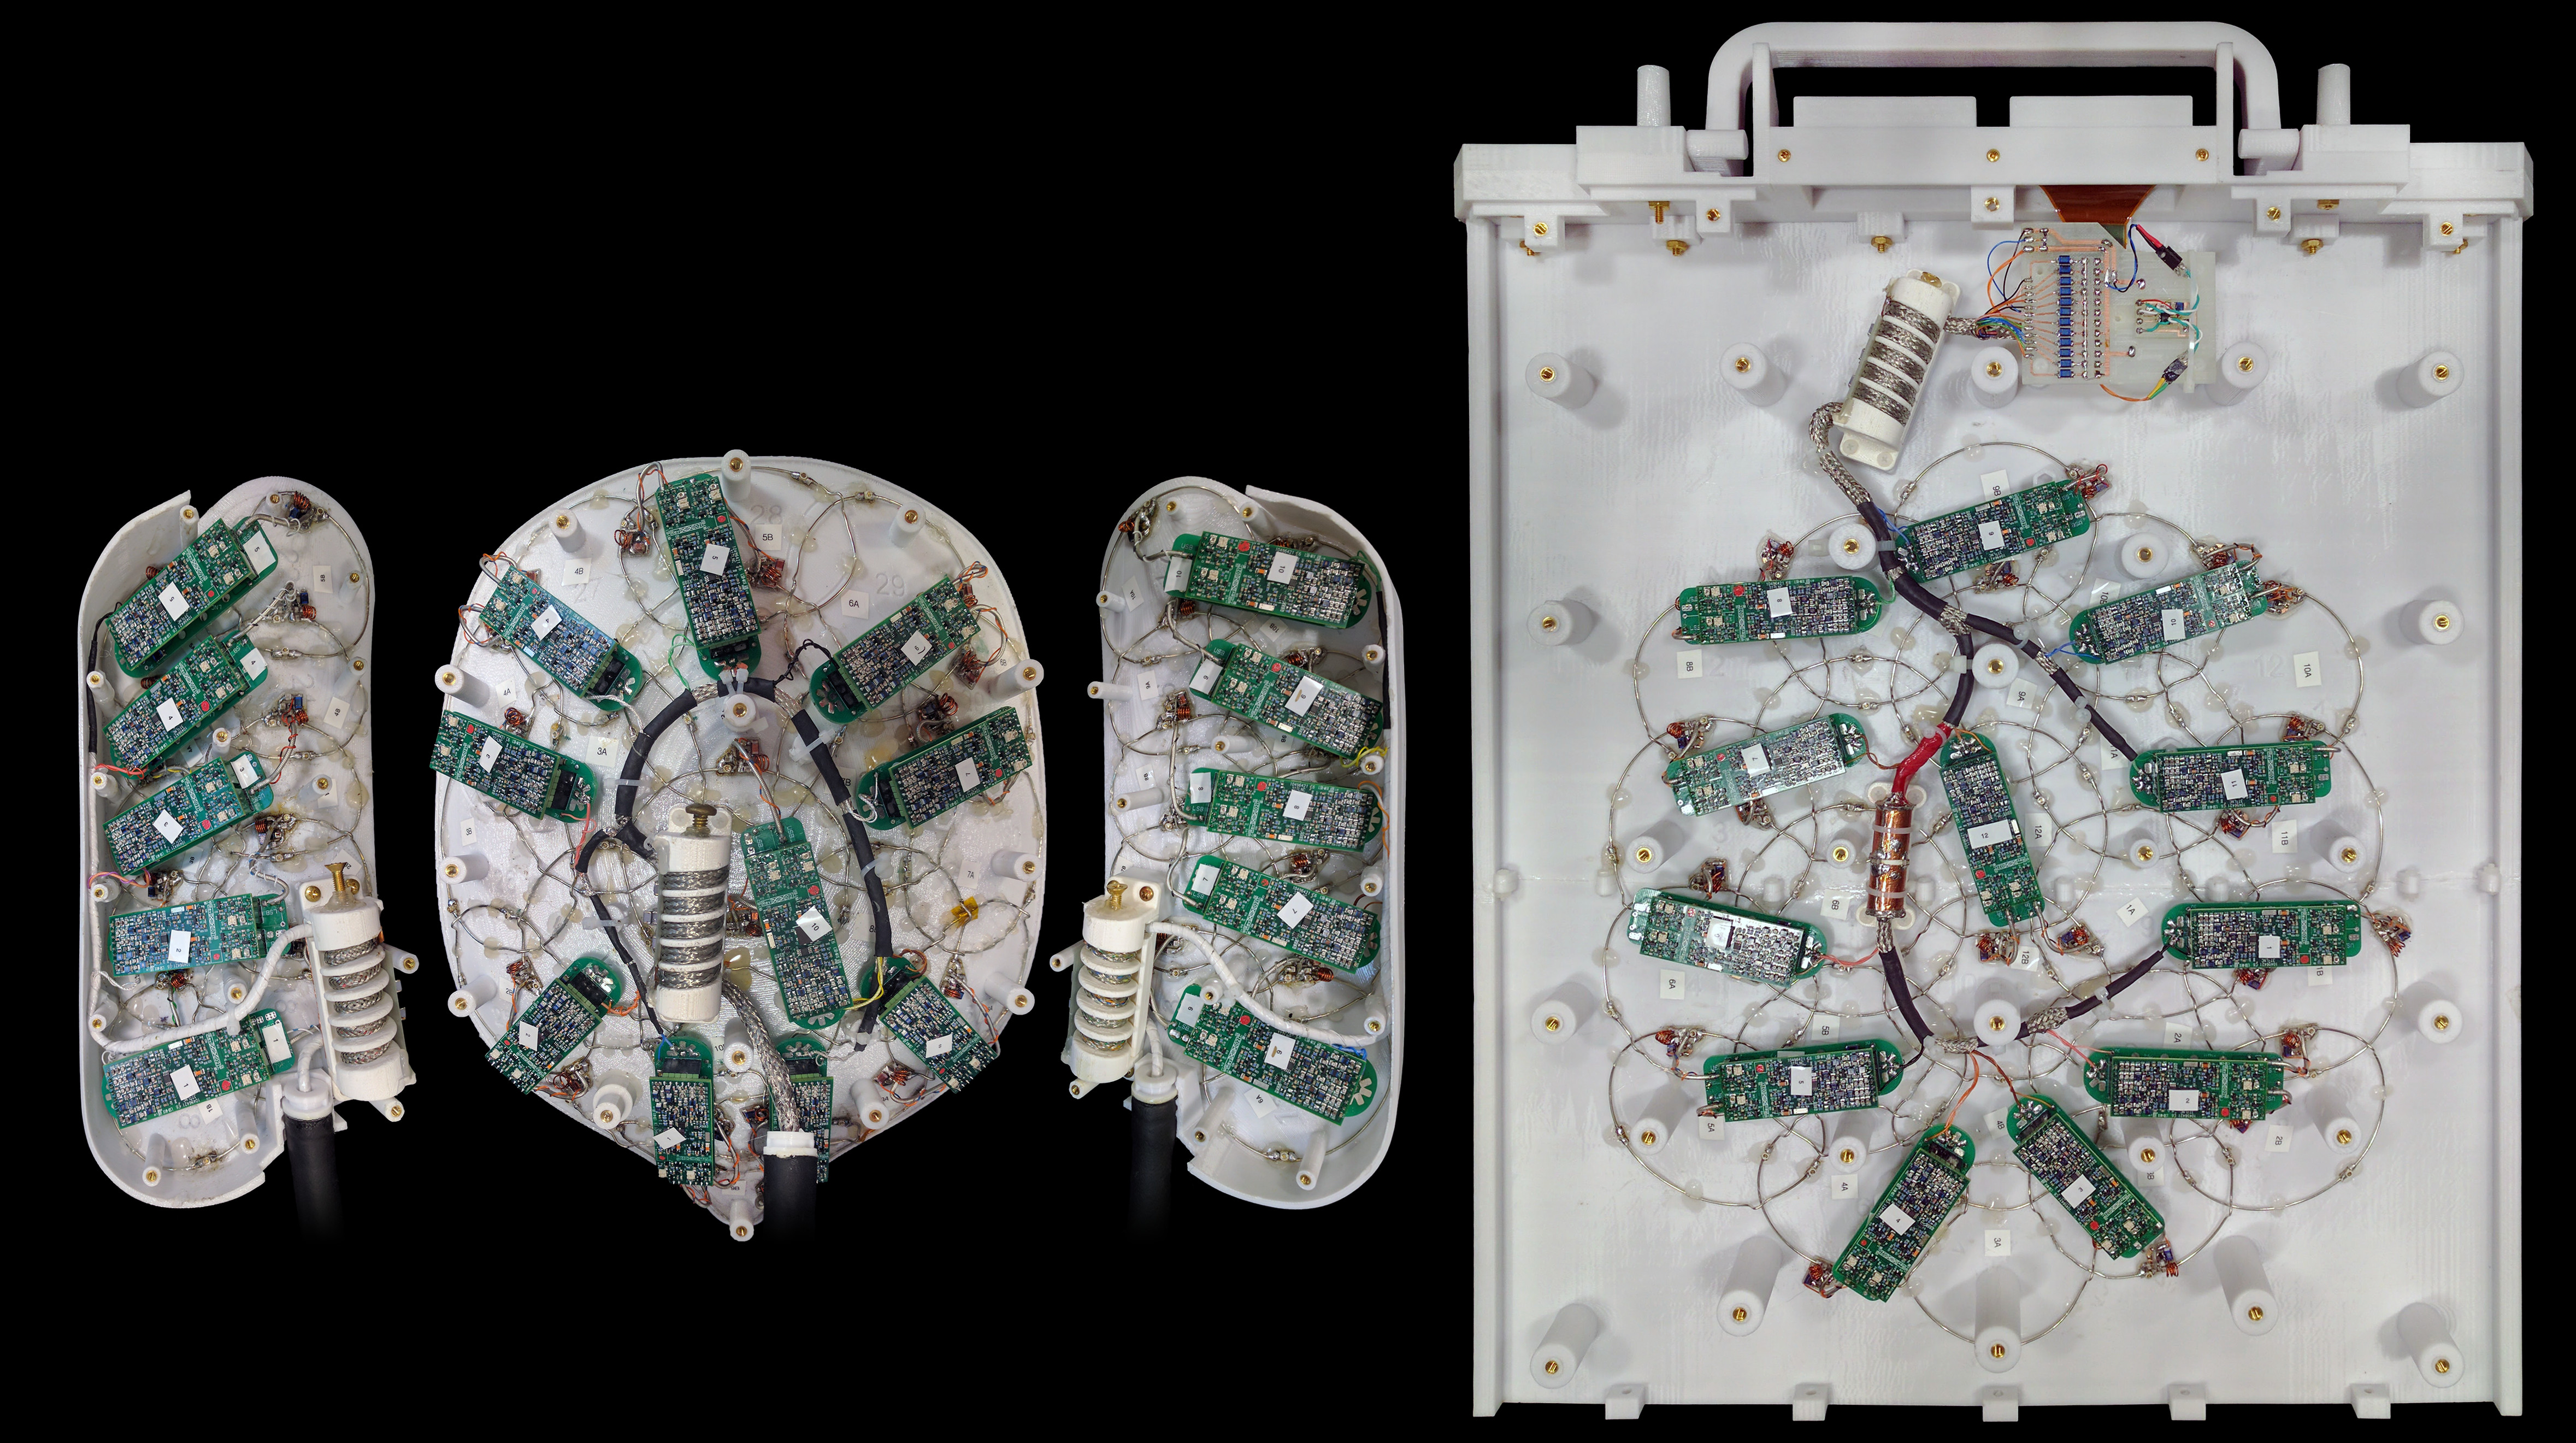
\includegraphics[width=6in]{figures/internals_composite.jpg}
\caption{View of internal coil construction}
\label{fig:internals_composite}
\end{figure}
\clearpage
\newpage

\begin{figure}
\vspace{2.4in}
\import{figures/}{loop_model.pdf_tex}
\caption{Loop circuit models}
\label{fig:loop_model}
\end{figure}
\clearpage
\newpage
